\tikzset{every picture/.style={line width=0.75pt}} %set default line width to 0.75pt

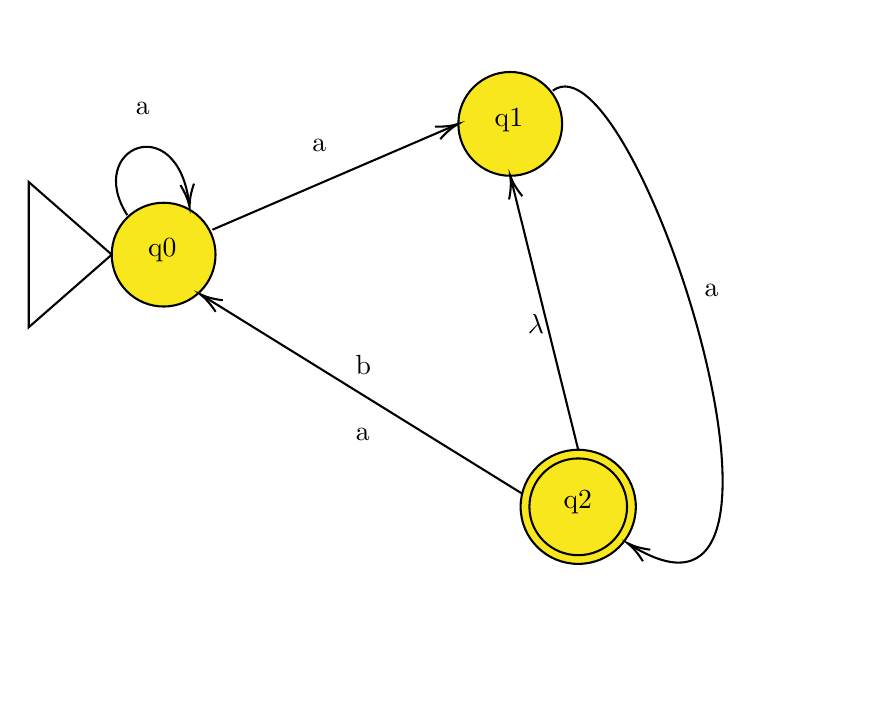
\begin{tikzpicture}[x=0.75pt,y=0.75pt,yscale=-1,xscale=1]
%uncomment if require: \path (0,777); %set diagram left start at 0, and has height of 777

%Flowchart: Extract [id:dp2213490168388459]
\draw   (48,96) -- (8,131) -- (8,61) -- cycle ;
%Shape: Circle [id:dp9156481012483882]
\draw  [fill={rgb, 255:red, 248; green, 231; blue, 28 }  ,fill opacity=1 ] (48,96) .. controls (48,82.19) and (59.19,71) .. (73,71) .. controls (86.81,71) and (98,82.19) .. (98,96) .. controls (98,109.81) and (86.81,121) .. (73,121) .. controls (59.19,121) and (48,109.81) .. (48,96) -- cycle ;
%Shape: Circle [id:dp8937236461295127]
\draw  [fill={rgb, 255:red, 248; green, 231; blue, 28 }  ,fill opacity=1 ] (215,33) .. controls (215,19.19) and (226.19,8) .. (240,8) .. controls (253.81,8) and (265,19.19) .. (265,33) .. controls (265,46.81) and (253.81,58) .. (240,58) .. controls (226.19,58) and (215,46.81) .. (215,33) -- cycle ;
%Shape: Ellipse [id:dp6295802993903136]
\draw  [fill={rgb, 255:red, 248; green, 231; blue, 28 }  ,fill opacity=1 ] (245,217.5) .. controls (245,202.31) and (257.42,190) .. (272.75,190) .. controls (288.08,190) and (300.5,202.31) .. (300.5,217.5) .. controls (300.5,232.69) and (288.08,245) .. (272.75,245) .. controls (257.42,245) and (245,232.69) .. (245,217.5) -- cycle ;
%Shape: Ellipse [id:dp23912526643664667]
\draw  [fill={rgb, 255:red, 248; green, 231; blue, 28 }  ,fill opacity=1 ] (249.23,217.5) .. controls (249.23,204.63) and (259.76,194.19) .. (272.75,194.19) .. controls (285.74,194.19) and (296.27,204.63) .. (296.27,217.5) .. controls (296.27,230.37) and (285.74,240.81) .. (272.75,240.81) .. controls (259.76,240.81) and (249.23,230.37) .. (249.23,217.5) -- cycle ;
%Straight Lines [id:da07722341343778594]
\draw    (245.5,211) -- (92.2,116.05) ;
\draw [shift={(90.5,115)}, rotate = 391.77] [color={rgb, 255:red, 0; green, 0; blue, 0 }  ][line width=0.75]    (10.93,-3.29) .. controls (6.95,-1.4) and (3.31,-0.3) .. (0,0) .. controls (3.31,0.3) and (6.95,1.4) .. (10.93,3.29)   ;
%Straight Lines [id:da5881939013667715]
\draw    (96.5,84) -- (213.16,33.79) ;
\draw [shift={(215,33)}, rotate = 516.71] [color={rgb, 255:red, 0; green, 0; blue, 0 }  ][line width=0.75]    (10.93,-3.29) .. controls (6.95,-1.4) and (3.31,-0.3) .. (0,0) .. controls (3.31,0.3) and (6.95,1.4) .. (10.93,3.29)   ;
%Curve Lines [id:da24978032388245308]
\draw    (260.5,17) .. controls (300.3,-12.85) and (399.5,298.86) .. (298.04,235.98) ;
\draw [shift={(296.5,235)}, rotate = 392.78999999999996] [color={rgb, 255:red, 0; green, 0; blue, 0 }  ][line width=0.75]    (10.93,-3.29) .. controls (6.95,-1.4) and (3.31,-0.3) .. (0,0) .. controls (3.31,0.3) and (6.95,1.4) .. (10.93,3.29)   ;
%Straight Lines [id:da3348378214953378]
\draw    (272.75,190) -- (240.48,59.94) ;
\draw [shift={(240,58)}, rotate = 436.07] [color={rgb, 255:red, 0; green, 0; blue, 0 }  ][line width=0.75]    (10.93,-3.29) .. controls (6.95,-1.4) and (3.31,-0.3) .. (0,0) .. controls (3.31,0.3) and (6.95,1.4) .. (10.93,3.29)   ;
%Curve Lines [id:da1693586185231678]
\draw    (55.5,77) .. controls (34.71,44.33) and (79.59,25.38) .. (85.34,71.58) ;
\draw [shift={(85.5,73)}, rotate = 264.05] [color={rgb, 255:red, 0; green, 0; blue, 0 }  ][line width=0.75]    (10.93,-3.29) .. controls (6.95,-1.4) and (3.31,-0.3) .. (0,0) .. controls (3.31,0.3) and (6.95,1.4) .. (10.93,3.29)   ;

% Text Node
\draw (247,123) node [anchor=north west][inner sep=0.75pt]   [align=left] {$\lambda$};
% Text Node
\draw (64,87) node [anchor=north west][inner sep=0.75pt]   [align=left] {q0};
% Text Node
\draw (231,24) node [anchor=north west][inner sep=0.75pt]   [align=left] {q1};
% Text Node
\draw (264.19,208.07) node [anchor=north west][inner sep=0.75pt]   [align=left] {q2};
% Text Node
\draw (58,21) node [anchor=north west][inner sep=0.75pt]   [align=left] {a};
% Text Node
\draw (332,109) node [anchor=north west][inner sep=0.75pt]   [align=left] {a};
% Text Node
\draw (143,39) node [anchor=north west][inner sep=0.75pt]   [align=left] {a};
% Text Node
\draw (164,143) node [anchor=north west][inner sep=0.75pt]   [align=left] {b\\ \\a};
\end{tikzpicture}
